\subsection{Prose Backend}\label{sec:prose} %0.5p
\begin{figure}[t]
\centering
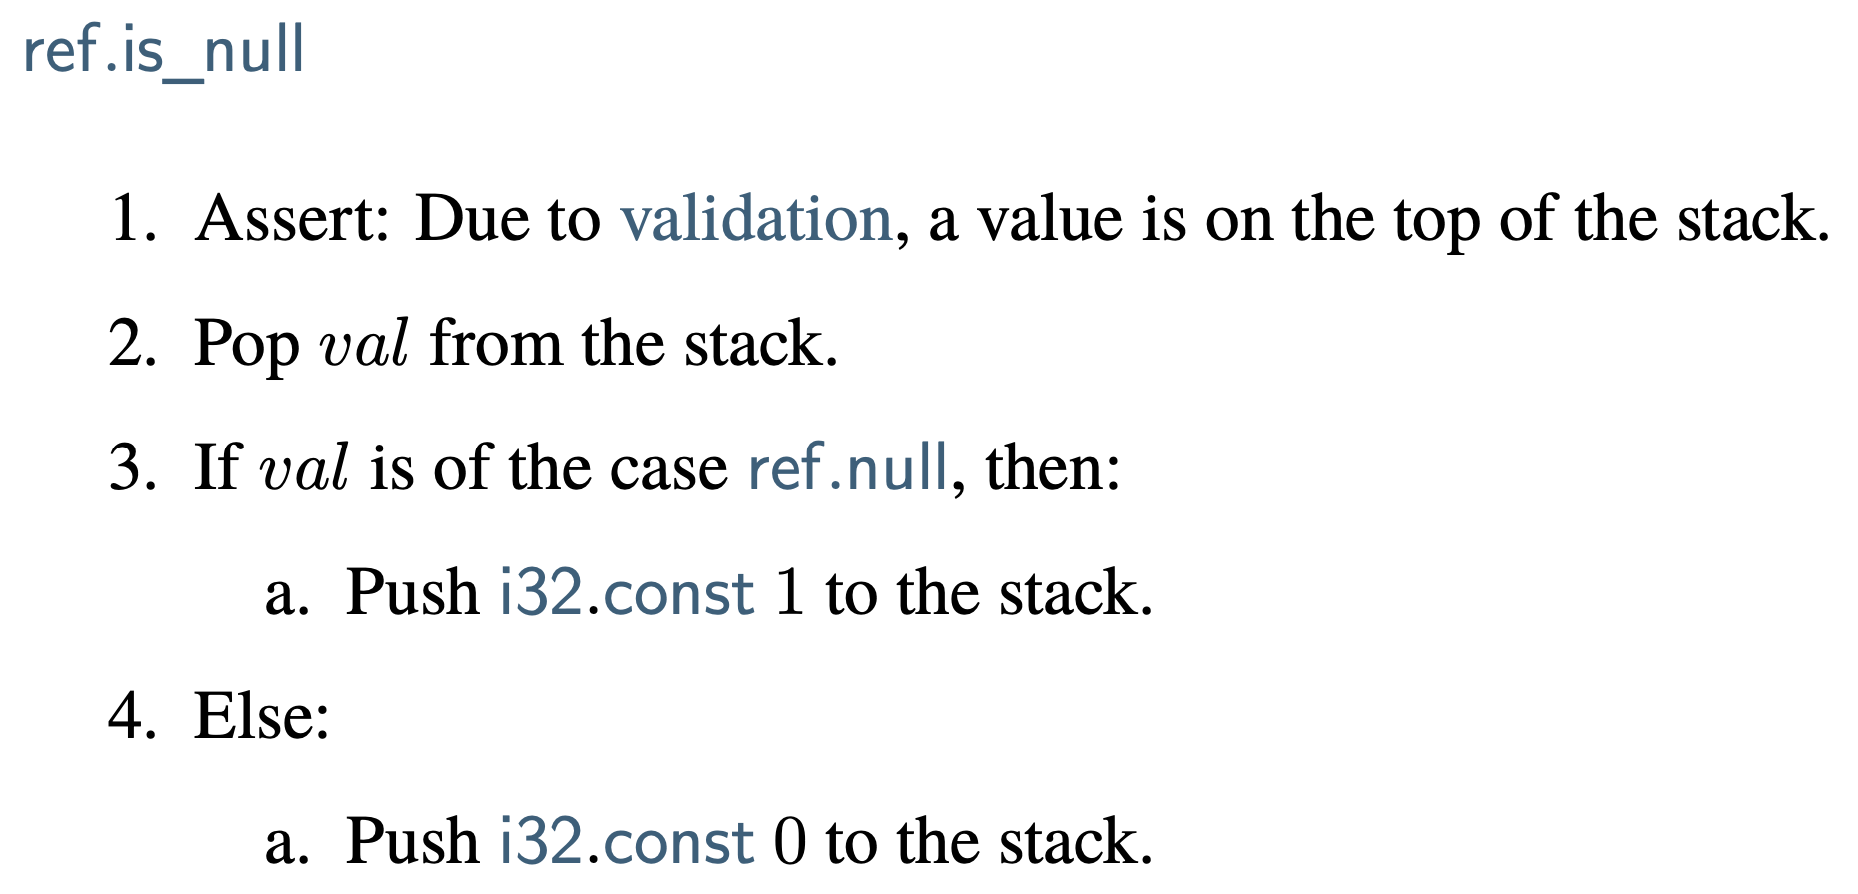
\includegraphics[width=.5\textwidth]{../img/genprose}
\vspace*{-1em}
\caption{Semantics of \inblue{\ensuremath{\mathsf{ref.is\_null}}} in a generated prose specification}
\label{fig:genprose}
\end{figure}

\al is designed to generate prose notation easily,
so the English prose specification can be generated directly from the semantics described in \al.
Fig.~\ref{fig:genprose} shows the prose pseudocode generated from the specification in Fig.~\ref{fig:dsl},
which is very close to the original handwritten prose description in Fig.~\ref{fig:spec1}.

\begin{itemize}
\item How to generate PDF with cross references
\item cf) error-prone generation of references done manually
\item systematic naming and bug detection?
\end{itemize}
